%\section{이론적 배경}

\section{연구 과정 및 방법}


\subsection{소형 천체망원경 자동화 시스템 구성}



%본 연구에서 사용되는 망원경은 기존 천체관측에 있어서 큰 어려움은 없어 원격 천체관측을 진행할 수 있어야 하며, 직접 덮개를 개발하게 되므로 적절한 크기를 가지고 있어야 한다. 최종적으로 선발된 망원경은 Takahashi 사의 'FSQ-106ED'이다. Takahashi 사의 웹사이트에서 참고한 FSQ-106ED의 스펙은 \textrm{Figure} \ref{FSQ}를 참고할 때 망원경의 경통은 580mm/675mm의 길이를 가지고 있으며, 지름은 125mm으로 마스크를 위한 덮개를 제작할 적절한 크기를 가지고 있다. Takahashi사의 FSQ-106ED의 사양 \cite{Godoy2018S}.

\begin{figure}[h]
	\begin{center}
		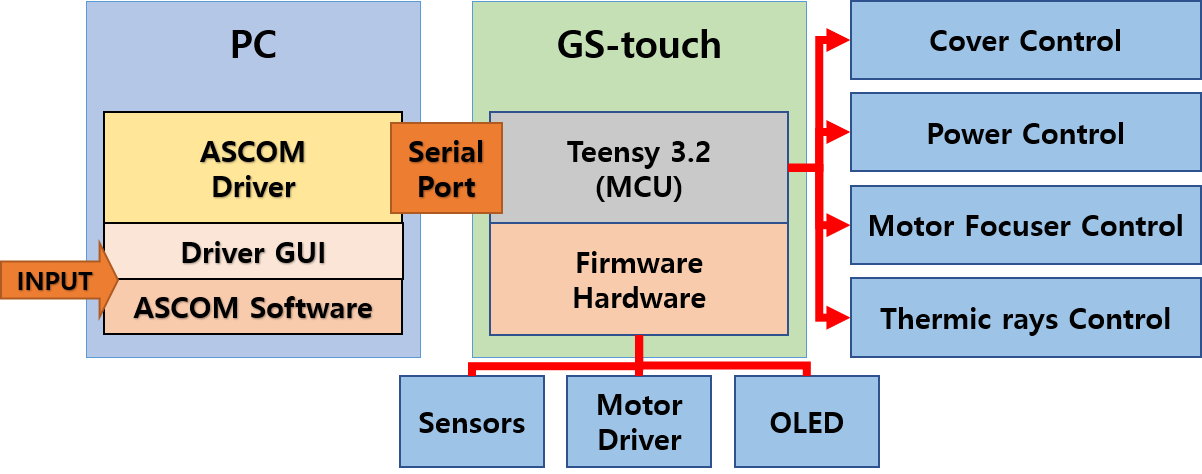
\includegraphics[width = 13cm]{GSsystem4}
	\end{center}
	\caption{GS-system의 대략적인 시스템 구성도}
	\label{GSsystem}
\end{figure}

소형 천체망원경을 자동화하기 위해서는 전원 스위치, 모터 포커서, 망원경 덮개, 이슬 제거용 열선 등이  제어되어야 한다. GS-system의 구동부에서는 모터 포커서와 망원경 덮개, 이슬 제거용 열선 등을 기존의 GS-touch를 보강한 Firmware를 개발하여, 명령을 통해 구동될 수 있도록 하였다. 이중에서도 전원 스위치(Power Control)은 여러 개의 전원을 한꺼번에 제어할 수 있도록 릴레이 스위치(Relay Switch)를 활용하였다.

제어부에서는 FocusMax와 같은 ASCOM 호환 소프트웨어에서 제작한 구동부를 제어할 수 있게 만들었다. 이를  위해서는 입력을 변환시켜주는 역할인 ASCOM 드라이버또한 업데이트할 필요가 있다. 외부에서 들어오는 입력은 ASCOM 드라이버를 통한 Serial Port를 이용하여 Firmware에 제어 명령으로 변환되는데, Firmware와 호환되는 명령을 내릴 수 있게 하기 위한 알맞은 입력을 PC를 통해 전달할 수 있도록 GUI를 추가로 제작하였다.



\subsection{구동부 제작}



\subsubsection{후드 제작}

후드는 Fusion360(https://www.autodesk.co.kr/products/fusion-360/students-teachers-educators)을 이용하여 \textrm{Figure}. \ref{fig:cover}와 같이 경통의 후드를 설계한 후, 3D 프린터로 출력하여 제작하였다. 경통의 후드는 천체망원경 별로 경통의 지름과 같은 특성이 다르고, 천체망원경 위에 고정시킬 수 있을 만큼 견고해야한다. 때문에 경통에 씌울 수 있도록 지름을 계산하여 팔각형 모양으로 감싸는 형태로 제작하였으며, 3D 프린터에서 출력할 수 있는 크기 제한이 있고 동시에 천체망원경에 부착시킬 때 편리하게 할 수 있도록 총 네 조각으로 나누어 조립하는 방식을 택하였다. 네개 조각의 렌치 볼트와 너트로 조립하여 완성할 수 있다.

본 연구에서는 부품들을 3D 프린터로 출력 후 조립하여 \textrm{Figure}. \ref{fig:cover}와 같이 이를 천체망원경의 후드처럼 부착시키는 것에 성공하였다. 후드의 지름은 망원경에 따라 달라질 수 있으므로 다른 망원경에 대한 후드를 제작할 때에는 이에 맞추어 새로 제작하여야 한다.

\begin{figure}[h]
	\begin{center}
		\begin{tabular}{cc}
			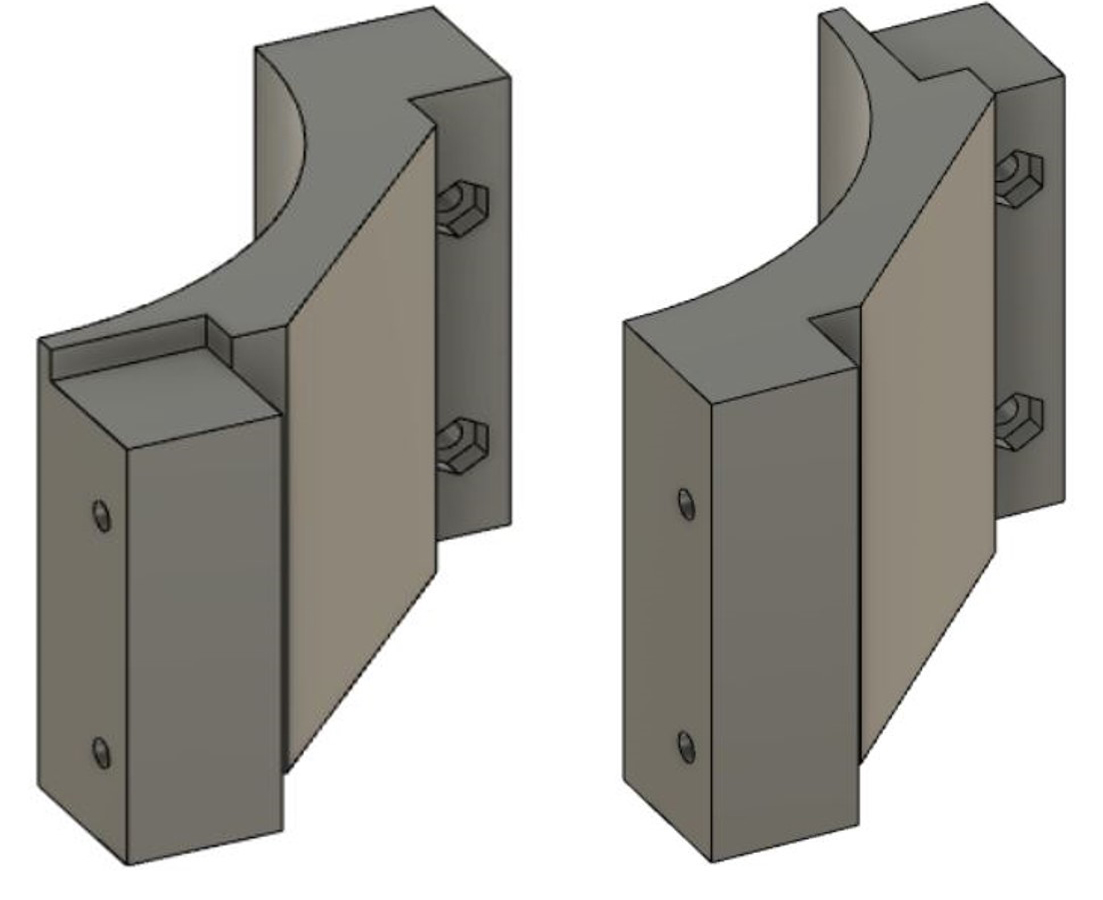
\includegraphics[width=5.8cm]{coverpeice} &   
			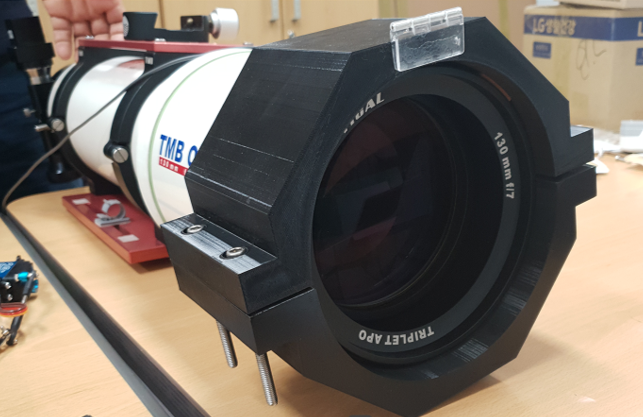
\includegraphics[width=7.5cm]{cover}
		\end{tabular}
	\end{center}
	\begin{tikzpicture} [remember picture,overlay]
	\node at (0.4, 5.2) {(a)};
	\node[text=white] at (7.0, 5.2) {(b)};
	\end{tikzpicture}	
	\caption{(a) Fusion360을 이용하여 설계한 경통 덮개 조각들, (b) 제작한 후드를 천체망원경에 장착한 모습.}	
	\label{fig:cover}
\end{figure}


\subsubsection{아크릴 덮개 제작}

천체망원경의 자동화를 실현하기 위해서는 경통의 덮개를 열고 닫는 것이 필요한데, 소형 천체망원경의 경우 이러한 기능이 개발되어 있지 않다. 천체망원경의 광학계는 사용하지 않을 때에는 먼지, 이슬 등의 피해를 최소화 하기 위하여 덮개를 덮어 두어야 하고, 관측시에만 덮개를 열고 관측하는 것이 바람직하다. 
\begin{figure}[h]
	\begin{center}
		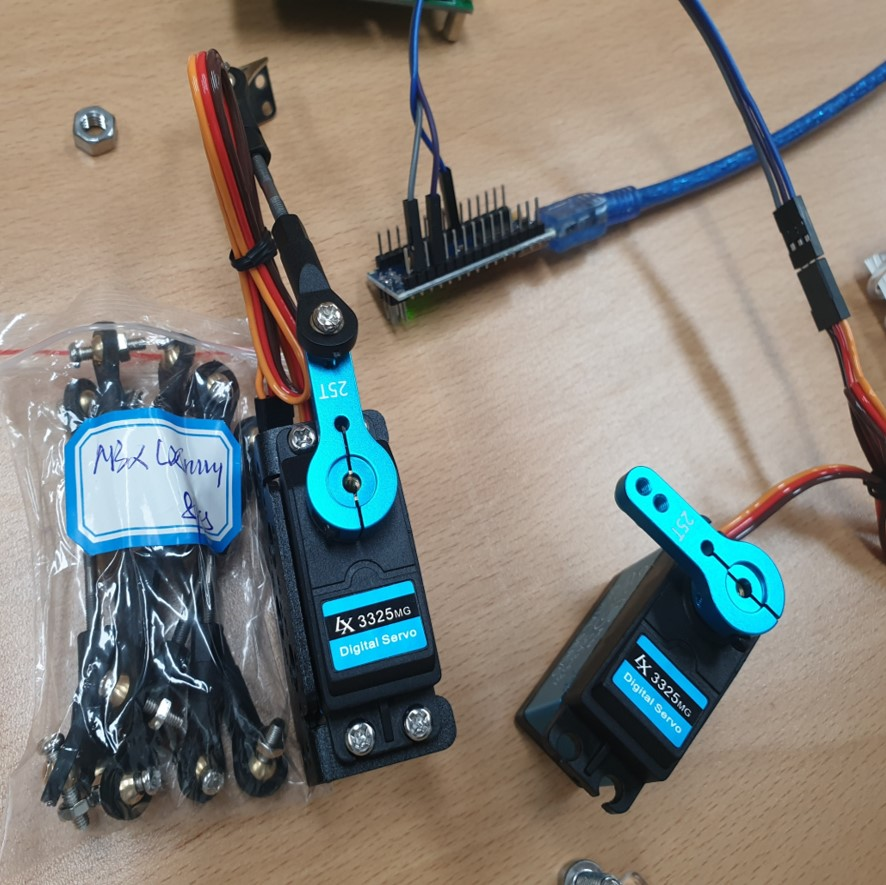
\includegraphics[width = 7cm]{servo1}
	\end{center}
	\caption{경통 덮개를 제어하기 위해 사용한 서브모터 ds lx3325mg 25kg}
	\label{motor}
\end{figure}


경통의 후드에서 바흐티노프마스크를 확실하게 제어하기 위해서는 바흐티노프마스크를 적용할 때와 적용하지 않을 때의 구분이 확실해야한다. 이를 확실하게 하기 위해서 바흐티노프마스크를 경첩을 이용하여 큰 각도로 제어하는 방법을 택하였으며, 이를 위해 덮개를 설계할 때 \textrm{Figure}. \ref{fig:cover}b와 같이 경첩의 높이를 고려하여 제작하였다.

서보모터는 일반적으로 사용하는 DC모터와 다르게 원하는 각도로 모터의 속도를 조절하여 이동시킬 수 있는 모터로,  RC카의 방향제어, 로봇의 관절제어 등의 상황에서 자주 사용되곤 한다. 본 연구에서 사용한 서보모터는 ‘ds lx3325mg 25kg’ 모델(\textrm{Figure}. \ref{motor})으로, 서보모터이지만 360도 회전이 가능한 모델으로, 몸체가 금속으로 되어있어 내구성을 기대할 수 있으며, 축이 톱니모양으로 되어 있기 때문에 제어가 편리하다는 장점을 가지고 있다.



\begin{figure}[ht]
	\begin{center}
		\begin{tikzpicture}
		\node[anchor=south west,inner sep=0] at (0,0) 
		{
			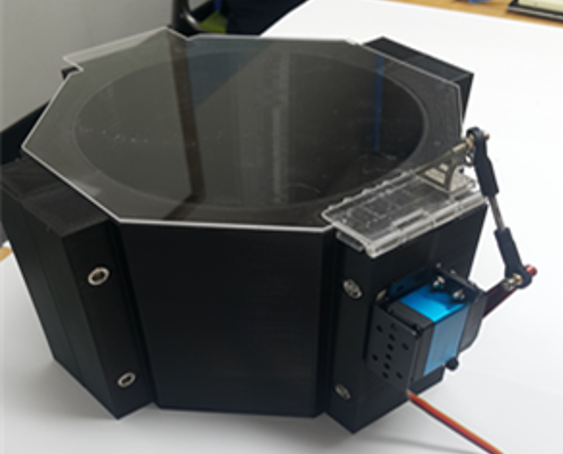
\includegraphics[height=4.5cm]{servo2}
			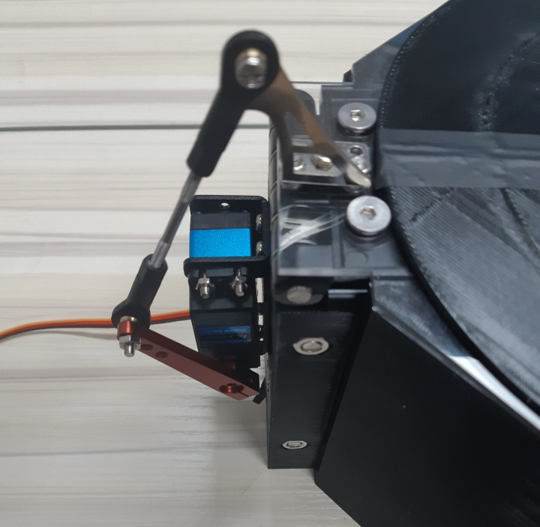
\includegraphics[height=4.5cm]{hinge} 
		};
		\draw (0.3, 4.2) node {(a)};
		\draw (6.1, 4.2) node {(b)};
		\end{tikzpicture}
	\end{center}
	\caption{(a)서보모터를 제작한 후드에 장착한 모습 (b) 개선한 경첩 및 서보모터}
	\label{servohinge}
\end{figure}

서보모터의 경우 구동을 위해 필요한 핀은 3가지이며, 일반적으로 주황색, 빨간색, 갈색의 핀으로 이루어져 있다. 주황색 핀은 모터를 제어할 수 있는 핀이며, 빨간색 핀과 갈색 핀은 각각 $\textrm{5 V}$ 전원과 GND에 연결하여 서보모터를 구동할 수 있다. 서보모터의 경우 \textrm{Figure}. \ref{servohinge}a처럼 후드의 옆면에 부착시켜 일정한 각도로 제어할 수 있게끔 설계하였다.

이에 제작한 후드에 꼭 맞는 크기로 아크릴을 가공하여 덮개를 제작한 경첩을 달아 서보모터로 열고 닫을 수 있도록 설계하였다. 처음에는 \textrm{Figure}. \ref{fig:cover}b와 같이 아크릴 경첩을 이용하였으나 내구성에서 문제가 있다고 판단되어 견고하게 제작하기 위하여 금속 경첩으로 교체하였다. 금속으로 제작된 경첩은 볼트로 체결하는 방식으로 후드와 안정적으로 결합할 수 있었으며, 내구성 또한 뛰어났기 때문에 서보모터로 열고 닫는데 문제가 없었다. \textrm{Figure}. \ref{servohinge}b와 같이 금속 재질의 경첩은 덮개와 아크릴 바흐티노프 마스크 사이를 납작볼트를 이용하여 연결할 수 있으며, 이는 접착제를 이용하여 붙이는 방법보다 간단하고 견고하게 조립되었다.


\begin{figure}[ht]
	\begin{center}
		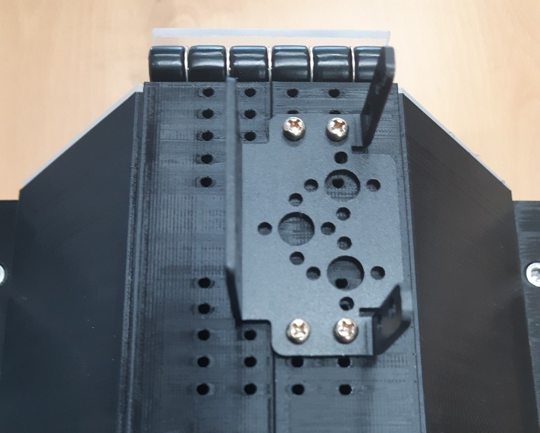
\includegraphics[width = 7cm]{servo3}
	\end{center}
	\caption{후드에 서보모터를 고정하기 위해 볼트를 이용해 고정한 모습}
	\label{servo}
\end{figure}


서보모터는 후드의 옆면에 부착시켜 제어한다. 이 때 정확한 위치에 부착시킬 수 있도록 일정한 간격을 두어 실험을 반복하였으며, \textrm{Figure}. \ref{servo}과 같이 적합한 위치를 찾아 고정시켰다. 서보모터로 마스크를 정확하게 제어하기 위해서는 마스크가 완전히 덮개에 고정될 수 있어야 하므로 이에 맞는 각도를 계산하여 사용하여야 한다.

\newpage
\subsubsection{바흐티노프마스크 제작}
천체망원경에 사용되는 대부분의 바흐티노프마스크의 도안은 직접 제작이 가능하며, 본 연구의 경우 Astrojargon (http://astrojargon.net/MaskGenerator.aspx) 사이트에서 망원경의 사양 및 마스크의 사용 목적에 맞는 적절한 바흐티노프마스크의 도안을 제작하여 사용하였다.

덮개에서 사용되는 방식을 이용한 바흐티노프마스크의 경우 기존처럼 종이나 알루미늄에 프린트된 방식일 경우 덮개에 원하는 모양으로 씌워지지 않을 가능성이 있다. 때문에 주변환경에 영향을 적게 받으면서도 그 면이 평평하여 천체관측을 진행할 때에 영향이 없어야 한다. 

\begin{figure}[h]
	\begin{center}
		
\includegraphics[width = 12 cm]{bendmask}
	\end{center}
	\caption{레이저에 의해 휘어진 아크릴 마스크}
	\label{bendmask}
\end{figure}


연구 초기에는 아크릴이 이러한 성질을 만족하면서도 쉽게 제작할 수 있으므로 아크릴에 레이저를 쐬여 바흐티노프마스크 모양을 씌우는 방법으로 테스트용 마스크를 제작해보았으나. 이러한 방식을 사용할 경우 \textrm{Figure}. \ref{bendmask}처럼 레이저로 인해 열을 받은 아크릴이 변형되어 정밀한 초점 조절이 불가능해지는 경우가 발생하였으며, 아크릴의 두께로 인해 실제로 초점을 조절할 때에 걸리는 여러 가지 변수 또한 무시할 수 없었다.

선택한 새로운 방법은 3D프린터를 이용하여 바흐티노프 마스크를 출력하는 것이다. 이 방법으로 얇으면서도 딱딱한 마스크를 사용할 수 있으므로 일반적인 아크릴을 활용한 마스크보다 적은 변수로 바흐티노프 마스크를 덮개에 부착시킬 수 있었다.

\begin{figure}[ht]
	\begin{center}
		\begin{tikzpicture}
		\node[anchor=south west,inner sep=0] at (0,0) 
		{
			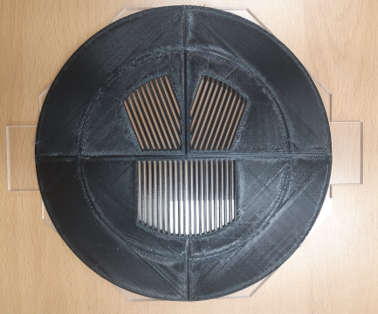
\includegraphics[height=4.5cm]{mask1}
			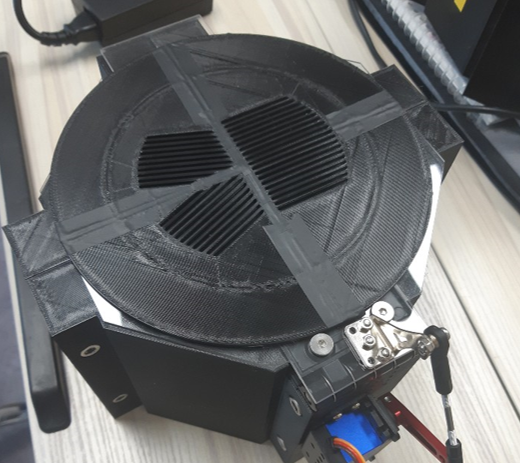
\includegraphics[height=4.5cm]{mask2} 
		};
		\draw (0.3, 4.2) node {(a)};
		\draw (5.9, 4.2) node {(b)};
		\end{tikzpicture}
	\end{center}
	\caption{(a) 4 조각으로 나누어서 출력한 FSQ-106ED 경통의 바흐티노프 마스크 (b) 출력된 마스크를 경통에 붙인 모습.}
	\label{mask}
\end{figure}

Astrojargon을 이용하여 출력한 바흐티노프마스크(\textrm{Figure}. \ref{mask})는 D값을 106, focal length 값을 530으로 출력하였으며, 덮개의 아크릴에 붙이기 편리하도록 지름을 아크릴과 같은 크기로 제작하였다. 출력 과정 중 바흐티노프마스크의 크기가 크기 때문에 4조각으로 나누어서 출력하였으며, 빛이 새는 것을 방지하기 위해 나중에 이를 검은 색 테이프로 봉합하였다. 

또한, 3D 프린터의 특성상 한쪽 면은 거친 면, 다른 한쪽 면은 평평한 면을 가지고 있다. 이 때 아크릴과 mask 사이의 거리를 일정하게 하기 위해 평평한 면이 아크릴과 같은 방향으로 올 수 있도록 고정시켰다.

\subsubsection{열선 제작}
\begin{figure}[h]
	\begin{center}
		\begin{tikzpicture}
		\node[anchor=south west,inner sep=0] at (0,0) 
		{
			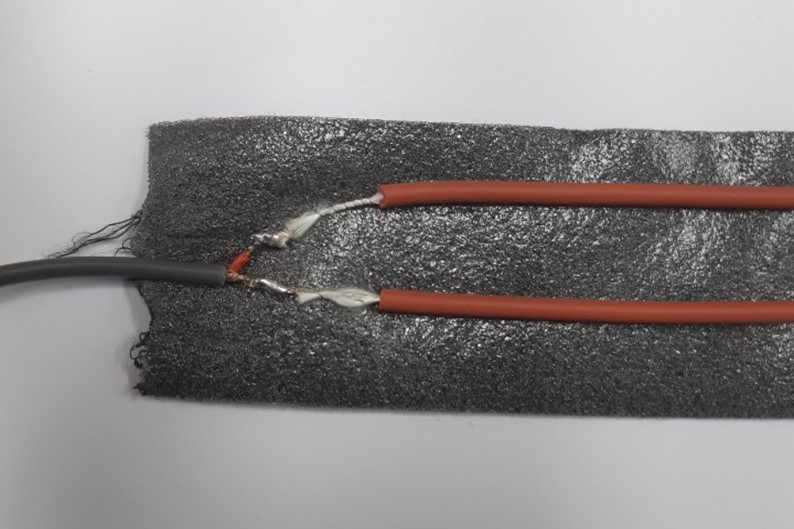
\includegraphics[width=6cm]{thermicline1}
			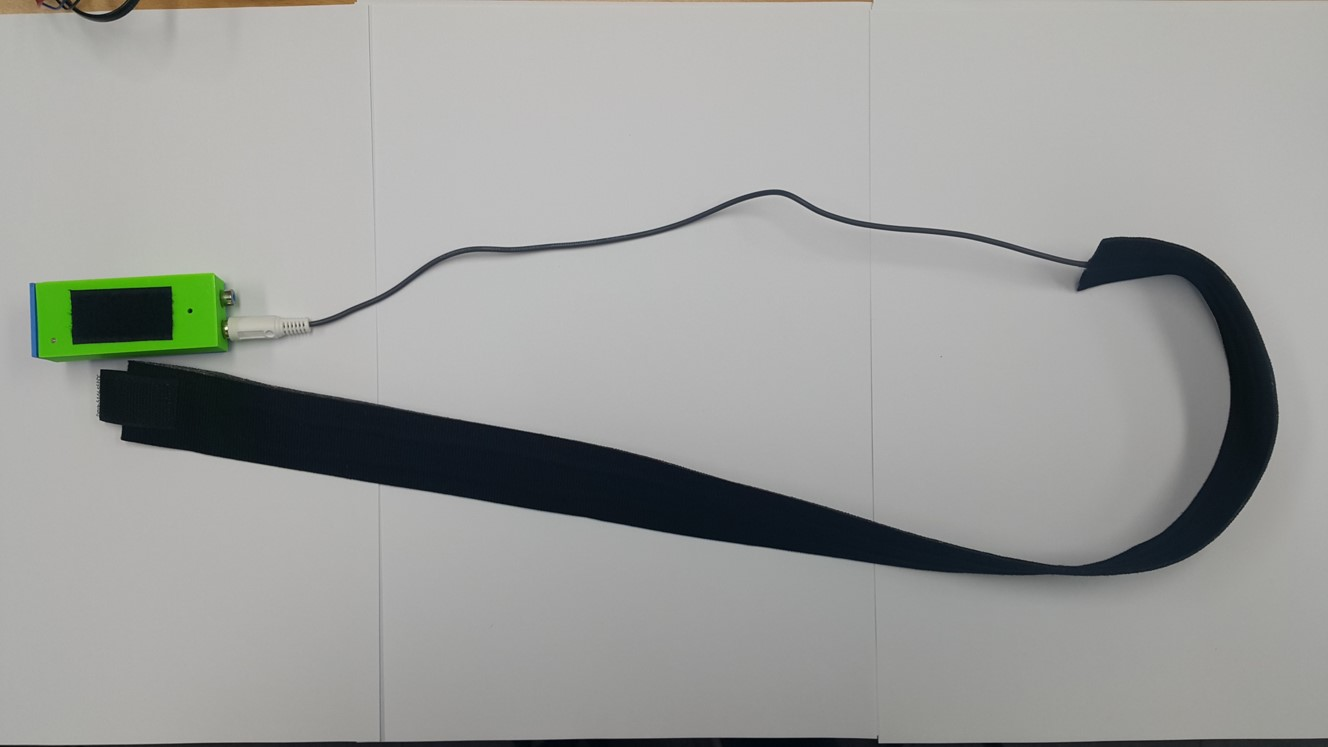
\includegraphics[width=7cm]{thermicline3} 
		};
		\draw (0.3, 3.7) node {(a)};
		\draw (6.4, 3.7) node {(b)};
		\end{tikzpicture}
	\end{center}
	\caption{(a) 제작한 열선의 접합부와 (b) 제작한 열선을 12V에 연결한 모습. 끝에 벨크로가 붙어있어 경통에 둘러 사용할 때 편리하다.}
	\label{thermic}
\end{figure}

열선은  니크롬선을 이용하여 제작하였으며, 망원경의 크기와 필요한 열량 등을 고려하여 니크롬선의 저항을 선택하였다.

열선 제작을 위해서 먼저 \textrm{Figure}. \ref{thermic}a처럼 끈끈한 면에 히팅케이블을 부착한 뒤에 알맞는 12V어댑터를 분해하여 극을 선과 연결한다. 그리고 열선을 다시 덮어주게 되면 12V 전원을 통해 작동하는 열선을 제작할 수 있다. 열선을 실제로 사용할 시에는 그 편의성을 증대시키기 위해 열선의 끝부분을 벨크로로 연결할 수 있도록 만들게 되며, 이렇게 제작한 열선은 렌즈가 있는 부분을 찾아 둘러주면 벨크로로 끝을 고정시켜 쉽게 망원경에 부착시킬 수 있다.

\newpage
\subsection{제어부 제작}

이전에 개발된 GS-touch는 바이폴라 스테핑 모터를 제어할 수 있는 모터 포커서로 초점 조절 기능과 이를 위한 기능들만이 주를 이루었기 때문에 보완할 필요가 있다. \textrm{Figure}. \ref{GStocuh}은 기존에 사용하는 GS-touch의 주요 기능들을 정리한 것이며, GS-touch는 전체적으로 두 가지 부분으로 나눌 수 있다.

\bigskip
\begin{figure}[h]
	\begin{center}
		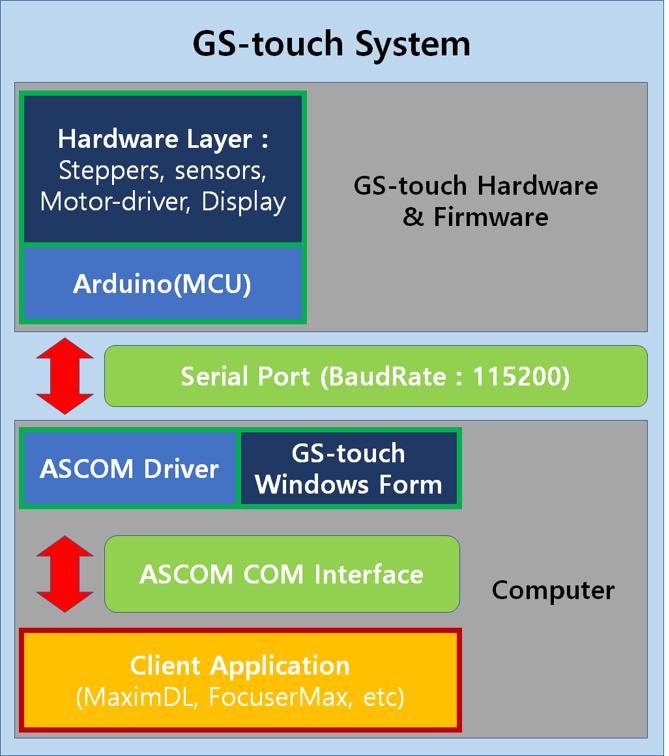
\includegraphics[width = 9.7cm]{GStouch}
	\end{center}
	\caption{GS-touch의 주요 기능}
	\label{GStocuh}
\end{figure}

첫 번째로 GS-touch의 Firmware는 모터를 직접적으로 제어할 수 있다. DRV8825 모터 드라이버를 활용하여 최대 1/32step의 마이크로 컨트롤을 지원하기 때문에 정밀하게 초점 위치를 찾을 수 있도록 설계되었으며 이들을 편하게 관리할 수 있도록 움직인 만큼의 step을 디스플레이에 나타내주며, 이를 원하는 숫자로 초기화하여 얼마나 더 움직였는지 또한 알기 쉽게 하였다. 부가적인 기능으로는 현재 컨트롤러의 위치의 온도와 습도를 알 수 있도록 하여 주변 상황을 쉽게 알 수 있도록 하였다.

두 번째 부분은 GS-touch의 직접적인 제어가 가능하도록 하는 ASCOM 호환 드라이버이다. GS-touch의 드라이버는 ASCOM 홈페이지에서 제공하는 개발자용 버전을 응용하여 C\# 기반으로 제작되었으며, GUI 및 애플리케이션 소프트웨어를 제공하기 때문에 펌웨어에서 제공하는 모든 기능들을 컴퓨터에서 원격으로 사용할 수 있도록 하였다.

비록 GS-touch는 여러 가지 기능을 가지고 있지만 천체망원경의 원격조작에 필요한 여러 기능들을 완벽하게 갖추지는 못하였다. 대표적으로, EEPROM을 사용하지 않았기 때문에 원하는 길이에 step값을 저장할 수 없으며, 온도 및 습도 측정 외의 편의기능 또한 없기 때문에 실제로 사용할 때 많은 불편함이 있다. 

본 연구에서는 이러한 단점들을 보완하여 EEPROM을 적용시키고 열선을 사용가능하도록 하는 등의 편의기능들을 개선하였으며, 이를 사용하여 소형 천체망원경의 자동화를 하고자 한다.

\subsubsection{회로 구성}

%\textrm{Figure} \ref{circuit01}와

\begin{figure}[h]
	\begin{center}
		%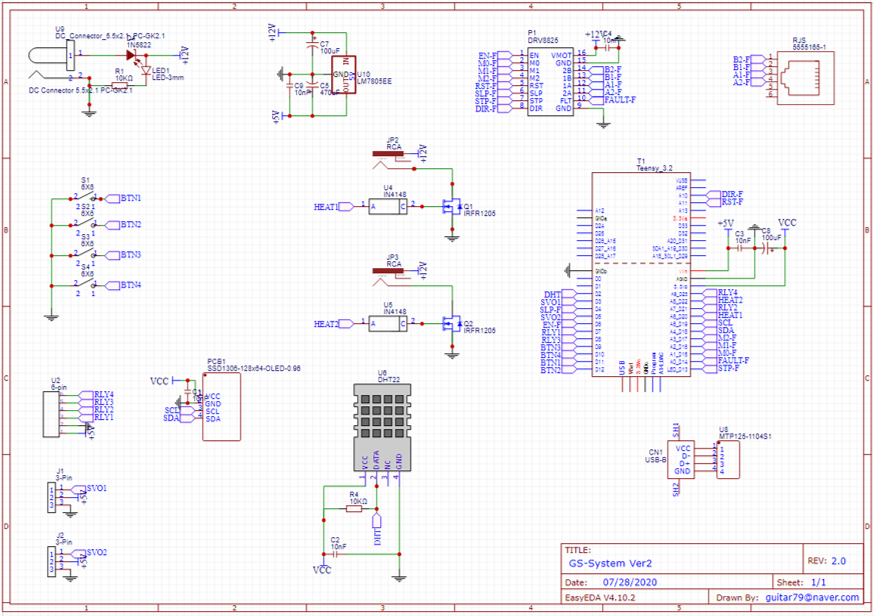
\includegraphics[width = 14.3cm]{circuit01}
	\end{center}
	\caption{Firmware하드웨어의 회로도}
	\label{circuit01}
\end{figure}
%https://easyeda.com/editor#id=be5835667e4c4db6afc5a1b05c65bfc7|757dc42a2f2e4ffe80eb74bb47231f57

\begin{figure}[ht]
	\begin{center}
		\begin{tikzpicture}
		\node[anchor=south west,inner sep=0] at (0,0) 
		{
			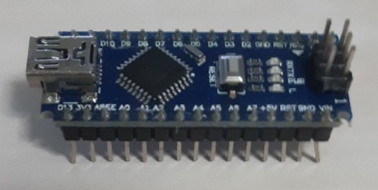
\includegraphics[height=3.5cm]{arduino}
			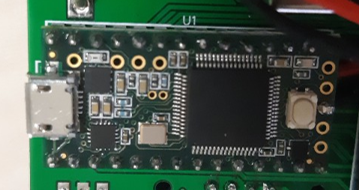
\includegraphics[height=3.5cm]{teensy} 
		};
		\draw (0.3, 3.2) node {(a)};
		\draw (7.4, 3.2) node {(b)};
		\end{tikzpicture}
	\end{center}
\caption{(a)GS-touch의 MCU인 Arduino Nano (b) 새로 제작한 Firmware 하드웨어의 MCU인 Teensy 3.2}
\label{mcu}
\end{figure}

 새로 만드는 Firmware의 하드웨어는 GS-touch와 다르게 여거가지를 제어해야 하므로 GS-touch에서 사용되었던 MCU(microcontroller unit)인 Arduino Nano (https://store.arduino.cc/usa/arduino-nano)보다 메모리 및 연산속도에서 더 강점을 가지면서 비슷한 크기를 가지고 있는 Teensy 3.2(https://www.pjrc.com/store/teensy32.html)를 활용하였다. 

반면에 Firmware의 소프트웨어는 기존과 비슷한 방법을 택하고 있는데, Serial을 통해 명령을 실행하는 함수와 함수에 입력할 값을 동시에 입력하면 제어키와 숫자로 이루어져 있는 기호를 통해 통신을 한다. 예를 들어, a에 모터 시계방향 회전을 담당하는 함수를 할당하고 a:100이라는 기호를 입력하면 모터는 시계방향으로 100step만큼 이동하게 된다. 모든 함수가 이러한 방법을 응용하였으며, 하드웨어의 버튼을 이용한 menu를 통해서도 함수의 일부분을 제어할 수 있도록 하였다.

\subsubsection{전원 제어}

릴레이 스위치는 전자석으로 이루어진 여러 스위치를 한번에 제어할 수 있도록 제작된 장비이다. 천체관측을 시작 및 종료할 때 가대, CCD, 카메라 등 한번에 여러 가지의 전원을 제어해야 하는데, 릴레이 스위치를 이용하면 한번에 제어할 수 있어 편리하다. 

\begin{figure}[h]
	\begin{center}
		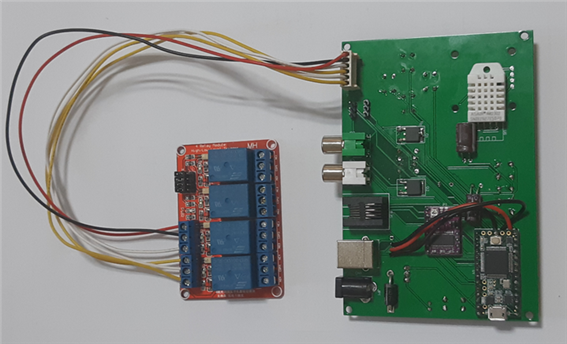
\includegraphics[width = 7.5cm]{relay}
	\end{center}
	\caption{실험에 사용된 릴레이스위치를 모터포커서에 연결시킨 모습}
	\label{relay}
\end{figure}


\textrm{Figure}. \ref{relay}와 같이 각각의 스위치를 선으로 연결시켜 MCU의 각 핀에 연결시켜 작동시킬 수 있으며, 함수로 지정하여 이들을 한번에 제어할 수 있도록 하였다.

릴레이 스위치는 6개의 핀으로 이루어져 있으며, 순서대로 $\textrm{+5 V}$, GND, 1, 2, 3, 4의 Relay이다. 때문에 각 핀들을 모두 연결시킨 뒤에 MCU를 이용하여 적절하게 제어할 수 있다. 각각의 기호는 P, Q, R, S이며, 상태만을 나타내기 때문에 서보모터 제어와 마찬가지로 오직 0과 1만을 입력받는다.



\subsubsection{서보모터 제어}
바흐티노프마스크를 제어하기 위해서 필요한 조건을 여러 가지가 있겠지만, 가장 중요한 조건 중 하나는 마스크를 사용하는 때와 그렇지 않을 때를 정확히 구분해야하며, 특히 마스크를 사용할 때에는 모든 상황에서 같은 환경을 제공할 수 있어야 한다. 본 연구에서는 경첩을 이용한 각도의 차이로 마스크를 제어하기 때문에 정확한 각도의 이동이 가장 중요하기 때문에 원하는 각도로 정확히 이동할 수 있는 서보모터를 사용하여 정확한 제어가 가능하도록 하였다.

일반적인 서보모터는 PWM을 응용하여 제어할 수 있으나, 대부분의 라이브러리에서 이미 그 값들을 적용시켜놓은 최적화 함수가 존재한다. 이를 활용하여 서보모터를 원하는 각도로 움직일 수 있도록 펌웨어 상에 코드를 제작하였다. 특히나 OLED를 활용하여 덮개에 부착된 마스크를 정확하게 제어할 수 있도록 하였다.

시리얼 포트를 통한 입력을 할 때 필요한 기호는 N이며, 오직 0과 1만을 입력받아 각각의 상태로 서보모터를 제어한다.

%\subsection{기존 모터포커서 보강}

%앞서 소개했듯이 기존의 모터포커서인 GS-touch는 모터의 초점을 맞추기 위한 기능들에 집중이 되어있기 때문에, 실제로 천체관측 및 원격 천체관측에서는 사용하기 아쉬운 부분들이 많았다. 이에 기존 모터포커서를 보강하였으며, 기존 모터포커서에 비해서 원격 천체관측에 필요한 여러 가지 기능들을 탑재하였다. 본 연구에서 새로 보강한 부분은 다음과 같다.

\subsubsection{열선 제어}
열선또한 정확한 천체관측에 필요한 장비 중 하나이다. 관측을 진행할 때에 경통의 온도가 내려가면 렌즈에 이슬이 맺히게 되는데, 이는 정확한 상을 맺히게 하는데 크게 어려움을 주게 된다. 열선을 경통에 감아놓으면 경통의 온도에 따라서 열선을 제어하여 깨끗한 렌즈를 사용할 수 있게되므로 관측을 편리하게 할 수 있으며, 때문에 천체망원경을 원격제어하기 위해서는 온도를 측정할 수 있는 장비와 열선이 필수적이다. 

열선은 PWM(Puls Width Modulation)을 이용하여 세기를 조절할 수 있다. PWM은 디지털 신호의 밀도로 그 세기를 조절하는 방식으로다 디지털 신호인 0과 1이 출력되는 시간의 비율을 조절하여 원하는 밀도로 제어할 수 있도록 한다. 본 연구에서 직접 제작한 열선을 포함한 대부분의 열선은 12V의 전압을 이용해 제어해야하기 때문에 아두이노의 출력 전원인 5V로는 신호만 제어하고 스위칭 트랜지스터를 이용하여 12V의 전압을 PWM으로 제어할 수 있도록 설계하였다.


\begin{figure}[ht]
	\begin{center}
		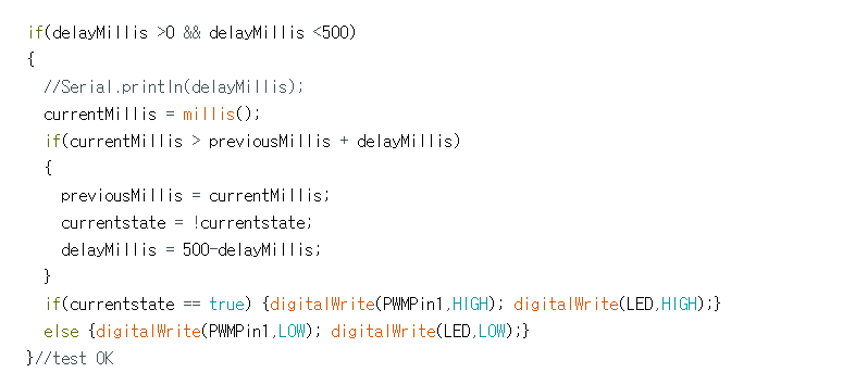
\includegraphics[width = 12.5cm]{PWMcode}
	\end{center}
	\caption{PWM제어를 위한 코드}
	\label{PWM}
\end{figure}


앞서 설명하였듯 열선의 제어는 전압의 PWM을 이용하여 실행된다. \textrm{Figure}. \ref{PWM}와 같이 시리얼 포트를 통한 입력을 할 때 필요한 기호는 A와 D이며, 0에이서 100사이의 값을 입력받아 500ms 주기로 값을 변화시킬 수 있도록 설계하였다.

\subsubsection{EEPROM(Electrically Erasable Read-Only Memory)}

MCU내에 원하는 값을 저장하는 방법은 여러 가지가 있다. 일반적으로 펌웨어가 실행되기 전에 변수를 선언하고, loop 문 속에 들어있는 여러 함수들을 통해 그 값을 바꾸는 방법을 사용하곤 한다. 하지만 원격 천체관측을 위한 펌웨어인 만큼, MCU내의 변수만으로 값을 저장하는 것은 상당히 위험하며, 그 전원을 계속 유지할 수 없기 때문에 다른 방법으로 값을 저장할 필요성을 느꼈으며, EEPROM은 기존 방법에 비해 안전하게 값을 저장할 수 있기 때문에 사용하게 되었다.


\begin{figure}[h]
	\begin{center}
		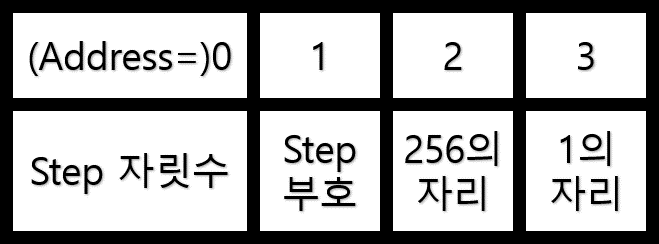
\includegraphics[width = 4cm]{eeprom1}
	\end{center}
	\caption{EEPROM의 address별 사용 구조. 부호와 값을 절대치를 이용하여 연산하였다.}
	\label{eeprom1}
\end{figure}


\begin{figure}[ht]
	\begin{center}
		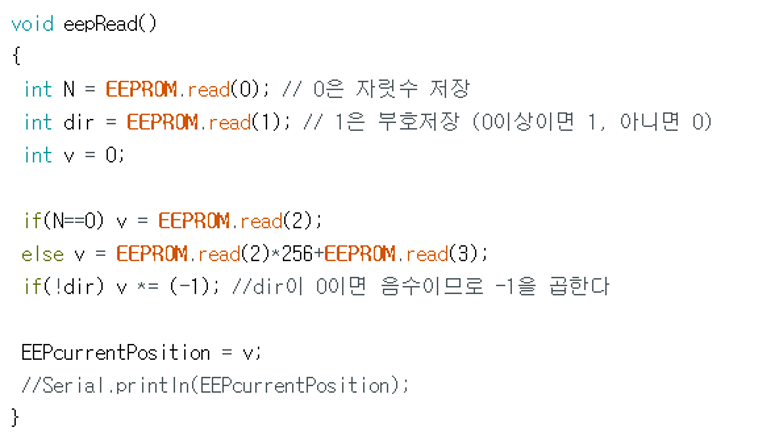
\includegraphics[width = 11cm]{eepread}
	\end{center}
	\caption{EEPROM에서 정보를 읽어오는 과정}
	\label{eepread}
\end{figure}

EEPROM은 대표적인 롬(ROM - read only memory)의 한 종류로서, 전원을 차단해도 저장된 정보를 유지하는 비휘발성 메모리이다. EEPROM은 address를 가지고 있어서 각각의 address 안에 지정된 bytes의 값을 저장할 수 있다. Teensy 3.2는 0에서 1023까지의 address지를 가지고 있고 하나의 address에 2048byte, 즉 0부터 255까지의 수를 저장할 수 있다. 모터포커서의 step을 저장하기 위해서는 약 100000범위의 수를 저장할 필요가 있다. GS-touch는 약 -50000에서 50000까지의 수를 저장할 수 있기 때문에 256진법을 활용하여 수를 저장할 수 있도록 설계하였다.


 모터포커서의 원활한 사용을 위해 저장되어야 하는 값은 모터의 위치를 저장할 수 있는 Position 값이다. \textrm{Figure}. \ref{eepread}은 값을 EEPROM에서 읽어오는 과정을 나타낸 것으로, 모터포커서가 최초로 실행될 때 EEPROM에서 값을 불러오고, 모터를 움직여 값을 변화시킨 직후에 적용된 값을 EEPROM으로 입력시키면 EEPROM값과 모터포커서의 Position 값을 항상 동기화시킬 수 있다.

%https://www.pjrc.com/teensy/td_libs_EEPROM.html

